\subsection{Documentación del proyecto}
La documentación juega un papel crucial en este proyecto, ya 
que proporciona una guía detallada sobre cómo utilizar los distintos 
componentes y plantillas disponibles. En este contexto, la adopción 
de Astro \cite{Astro} como herramienta para la generación de documentación
automática se debe a su facilidad de uso, ya que permite crear
páginas de forma sencilla utilizando Markdown, lo que facilita la
creación de documentos por los distintos integrantes del equipo.
Ya existen proyectos que han utilizado Astro para la generación
de documentación, como Microsoft con su proyecto Fluent UI 
\cite{astroPagesHalf}.\medskip

Concretamente, el proyecto usa Starlight, una plantilla de Astro que
proporciona una estructura de documentación predefinida, lo que
facilita la creación de documentación de forma rápida y sencilla.
Además, Starlight incluye un sistema de búsqueda y organización
de documentación, lo que facilita la navegación y búsqueda de
información en la documentación. Otra de sus ventajas es la
facilidad de customización, ya que permite modificar la apariencia
utilizando CSS o Tailwind e incluso incorporar funcionalidades
propias mediante JavaScript.

\subsubsection{Guías y manuales}
Para facilitar la integración de sistemas complejos como el aquí
propuesto, es necesario proporcionar guías que expliquen
de forma detallada cómo se debe interactuar con los diferentes
procesos. En este sentido, la documentación del proyecto incluye
un apartado de guías y manuales que proporciona esa información
de forma detallada. Además, se incluyen ejemplos de uso y casos
prácticos que ayudan a entender cómo se deben utilizar los distintos
elementos de forma interactiva y dinámica.\medskip

En este momento, la documentación incluye las siguientes guías:
\begin{itemize}
    \item \textbf{Guía de introducción:} proporciona una visión general del
    proyecto y qué partes lo componen.
    \item \textbf{Guía de instalación:} explica cómo instalar las diferentes 
    herramientas en local y conseguir acceso a los servicios. 
    \item \textbf{Guía de plantillas y componentes:} proporciona información detallada sobre cómo
    utilizar los distintos componentes y plantillas disponibles.
    \item \textbf{Guía de ClearMl:} introducción a la plataforma MLOps ClearMl y cómo
    utilizarla en el proyecto.
    \item \textbf{Guía de contribución:} proporciona información sobre cómo
    contribuir al proyecto y cómo colaborar con otros miembros del
    equipo.
\end{itemize}

En el futuro, se espera ampliar la documentación con nuevas guías
que no solo expliquen cómo utilizar los distintos elementos sino que
también se centren en aspectos enfocados a la IA y el aprendizaje
automático, como por ejemplo guías sobre cómo solucionar problemas
relacionados con el día a día de la empresa.

\subsubsection{Documentación de componentes y plantillas}
Todos los componentes y plantillas que forman parte del proyecto
cuentan con su propia documentación asociada a un archivo Readme.md.
La razón de utilizar un archivo de tipo Markdown es que es un formato
sencillo y fácil de escribir, lo que facilita la creación de documentación
por parte de los distintos integrantes del equipo. Además, Astro
lee de forma nativa archivos Markdown, lo que permite cargar las
diferentes páginas sin necesidad de escribir código propio de una
página web.\medskip

Aunque la documentación de los componentes y plantillas es bastante
flexible y permite incluir secciones adicionales si fuera necesario,
lo cierto es que por defecto incluye las siguientes secciones de forma
automática:

\begin{itemize}
    \item \textbf{Descripción:} proporciona una descripción general del
    componente o plantilla.
    \item \textbf{Instalación:} explica cómo instalar el componente o plantilla
    en un proyecto. Generalmente, se proporciona un único comando de consola que
    instala el componente o genera la estructura de archivos de la plantilla. 
    \item \textbf{Uso:} proporciona información sobre cómo utilizar el componente
    o plantilla en un proyecto. Incluye ejemplos de uso.
    \item \textbf{Tags:} lista las etiquetas que se han utilizado para indexar en
    el sistema de búsqueda.
\end{itemize}


\subsubsection{Sistema de búsqueda y organización de documentación}
El poder encontrar información de forma rápida y sencilla es crucial
en un proyecto de estas características, ya que la documentación
puede llegar a crecer significativamente dificulta encontrar
la información relevante. Una de las ventajas de Astro con Starlight
es que proporciona de forma automatizada un sistema que permite realizar 
búsquedas en base a palabras clave.\medskip

El sistema que utiliza por detrás se llama Pagefind \cite{Pagefind}, el cual es gratuito 
y de código abierto. Pagefind es un motor de búsqueda de documentos
que entre sus características incluye no solo la búsqueda por palabras
clave sino también el filtrado de resultados mediante etiquetas, se puede observar
un ejemplo en la figura \ref{fig:search-menu}. Esta 
funcionalidad es clave y permite encontrar la información de forma más precisa. 
Para poder indexar los documentos, Pagefind necesita que estos cuenten con
unas etiquetas especiales que le permitan identificar que cierto documento
pertenece a una categoría en concreto. En este sentido, ciertas páginas
de la documentación cuenta con una sección llamada \textit{Tags} en la que
se incluyen las etiquetas correspondientes.\medskip

\begin{figure}[!h]
    \centering
    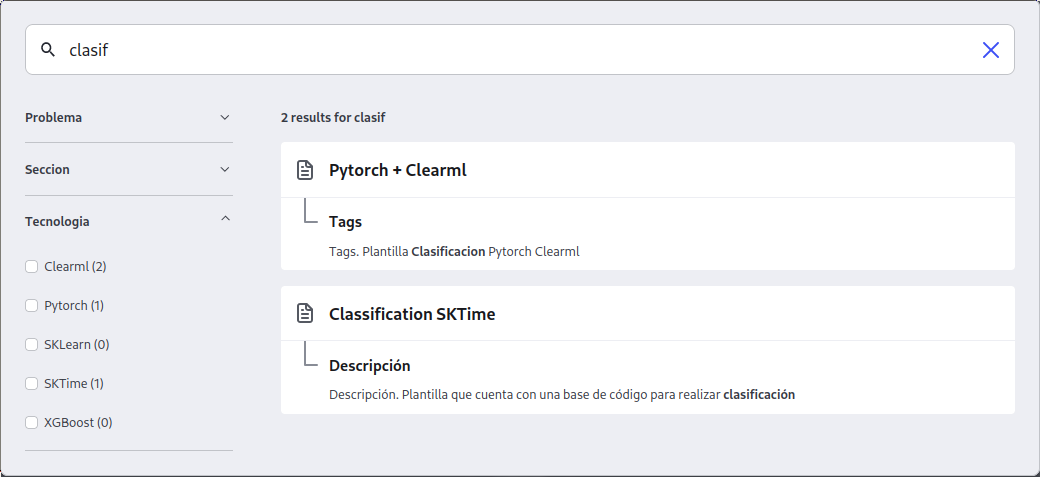
\includegraphics[width=\textwidth]{search-menu.png}
    \caption{Sistema de búsqueda}\label{fig:search-menu}
\end{figure}

Aunque de momento el sistema de búsqueda funciona correctamente, se
espera en un futuro poder cambiar el motor que utiliza Astro por defecto 
a uno que permita búsquedas más enfocadas en la semántica
de los documentos y no solo en base a palabras clave. Una alternativa que
se están considerando podría ser Algolia \cite{algoliaWhatAlgolia},
un motor impulsado por IA muy popular dentro del mercado. El
problema de Algolia es que es un servicio de pago, por lo que se
debería estudiar si merece la pena ese coste adicional o si se
existen alternativas gratuitas que ofrezcan un servicio similar y
sean mejores que Pagefind.

\subsubsection{Construcción automática de documentación}
Como se ha mencionado anteriormente, cada componente y plantilla 
viene con su propia documentación, la cual se genera dentro de su
respectiva carpeta mediante un archivo Readme.md. La decision de 
que cada componente tenga su documentación en su propia carpeta
es para facilitar la experiencia de desarrollo ya que todos los
elementos de cada componente se encuentran en un mismo lugar y no
es necesario buscar en diferentes carpetas para encontrar la
información necesaria.\medskip

Esto, pese a ser una ventaja, también genera un problema a la hora de
generar la documentación, ya que es necesario un sistema que sea
capaz de recorrer todas las carpetas, extraer los archivos Readme.md
y Readme.mdx de cada una de ellas y generar la respectiva página
de documentación. Para solucionar este problema, se ha creado un
script de bash que recorre las carpetas que contienen componentes o
plantillas y copia estos archivos en una carpeta con el nombre de
su carpeta original con el fin de evitar problemas de colisiones
entre los nombres de los diferentes archivos. Una vez hecho esto,
se ejecuta el comando astro build y se sube la documentación a la
plataforma de GitLab Pages.

